\subsection{Results and Analysis} \label{Result section}

Table \ref{Experiment summary table} states all the combinations of ansatzes and methods.

The two ansatzes' \emph{NLocal} and \emph{TwoLocal} gradient variances decay as expected for the unrestricted setting.
Their decay rate is exponentially fitted with the rate of -0.65 and -0.72 respectively.
The figure \ref{Plot ansatzes variance default} shows the results of the two ansatzes in this configuration.
The semi-log plots portray the variances of gradient from differences ansatzes in the unrestricted configuration.
Consider that the unit measure for variance is in \emph{exponential} form, so the linear graph is exponentially closer to zero for each qubit added to the circuit.
This result indicates that the cost function landscape becomes flatter and flatter.
Eventually, the gradient would reach a near-zero value across a large plateau, which would be inefficient for any gradient-based optimization algorithm to train the model.
We discussed this phenomenon in Section \ref{Barren Plateaus section}.


\begin{figure}
    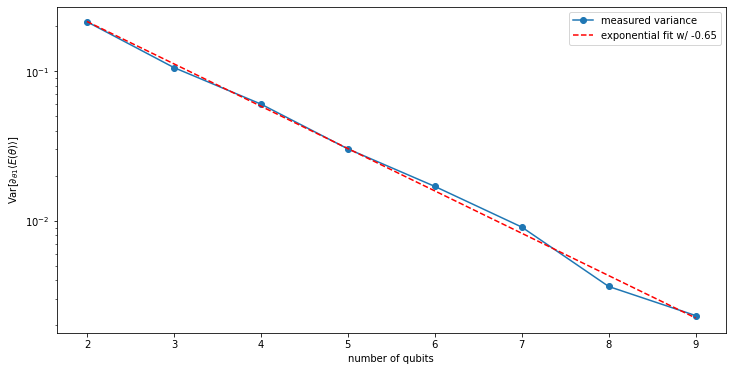
\includegraphics[width=\textwidth]{Artefact/Appendices/NLocalDefault.png}
    \centerline{a) NLocal Ansatz gradient variance values}
    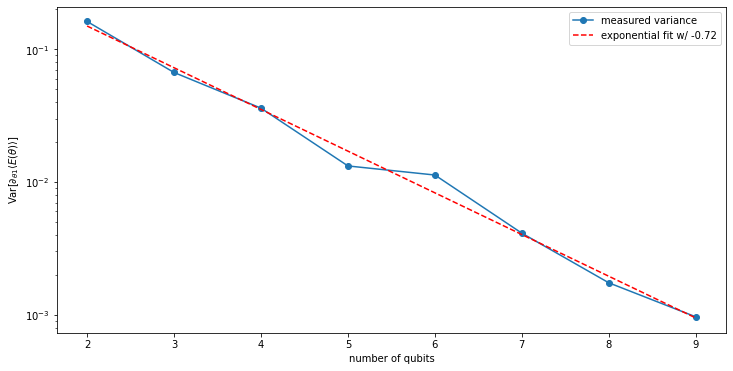
\includegraphics[width=\textwidth]{Artefact/Appendices/TwoLocalDefault.png}
    \centerline{b) TwoLocal Ansatz gradient variance values}
    \caption{
        The variances of gradient from differences ansatzes in the default configuration, the circuit is measured as a global cost function.
        For each iteration, we increase the qubit and repetition count by 1, starting from 2 to 9.
        The variances vanish exponentially to the number of qubits.
    }
    \label{Plot ansatzes variance default}
\end{figure}

In contrast, for the case of Local Cost Function and Shallow circuit, we observe that the variances of the ansatzes' gradient did not vanish when we attempted to increase the number of qubits.
The slope of the ansatzes \emph{NLocal} and \emph{TwoLocal} in this case decay exponentially fit with -0.07 and -0.04 respectively.
This implies that the cost function landscape can sustain the slope.
Figure \ref{Plot ansatzes variance local cost} shows the result of the experiment for local cost function and shallow circuit.
We can see that the NLocal ansatz case produced a more steady graph compared to the TwoLocal ansatz, which mean the trainability of gradient-based optimization algorithms would be consistent.
For TwoLocal ansatz, we can see that the graph is more unstable. 
For example, the variance value for 7 qubits is higher compared to 4 or 9 qubits.

\begin{figure}
    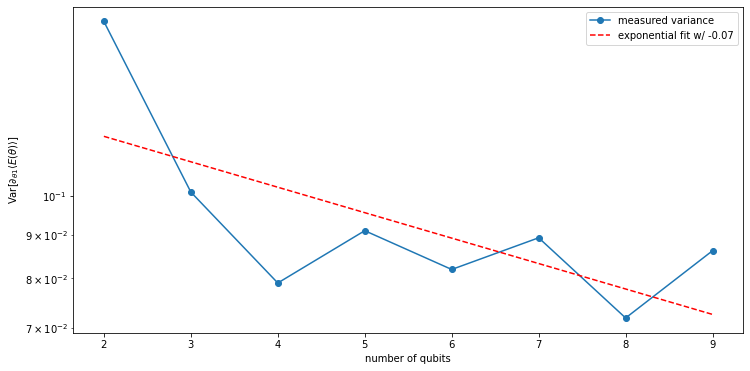
\includegraphics[width=\textwidth]{Artefact/Appendices/NLocalFixedLocal.png}
    \centerline{a) NLocal Ansatz gradient variance values}
    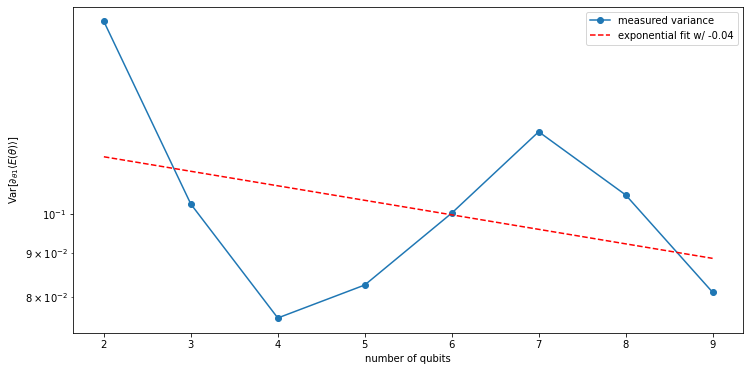
\includegraphics[width=\textwidth]{Artefact/Appendices/TwoLocalFixedLocal.png}
    \centerline{a) TwoLocal Ansatz gradient variance values}
    \caption{
        The variances of gradient from different ansatzes after applying a local cost function.
        We plot 2 to 9 qubits while keeping the repetition value fixed as 1.
    }
    \label{Plot ansatzes variance local cost}
\end{figure}

To compare the effectiveness of the local cost function treatment, we plot the variance graph of above mention cases in Figure \ref{Plot variance default and Local Cost} and the Table \ref{Experiment summary table}.
The results have shown the differences in the decay rates of different ansatzes and methods.
Overall, the ansatzes with the local cost function and restriction on circuit depth have their variance values remaining higher and being more consistent for higher qubit count. 
The ansatz with this treatment, therefore would not possess a barren plateau.
On the other hand, the values for the default cases shrink exponentially and eventually, the near-zero gradient around the initial point will expand to a large plateau.



\begin{figure}
    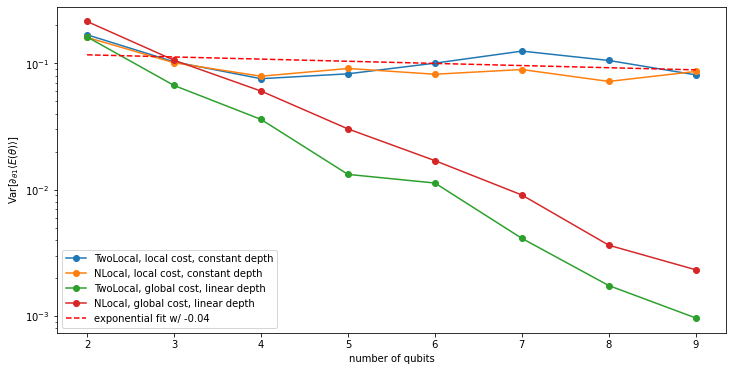
\includegraphics[width=\textwidth]{Artefact/Appendices/variancesLCF.png}
    \caption{
        Comparison of the variance values of the two ansatzes with and without Local Cost Function and constant depth.
        The ansatzes with Global Cost Function and unrestricted depth have their gradient variances decay exponentially with the number of qubits.
    }
    \label{Plot variance default and Local Cost}
\end{figure}
